\documentclass[11pt,a4paper]{article}
\usepackage[T1]{fontenc}
\usepackage[latin1]{inputenc}
\usepackage{lmodern}
\usepackage{float}
\usepackage{a4wide}
\usepackage[dvips]{graphicx}

\usepackage[
pdfauthor={ACE Project Team},
pdftitle={Developers Guide},
pdfcreator={pdftex},
]{hyperref}

\usepackage{sectsty}
\allsectionsfont{\sffamily}

\usepackage{fancyheadings} 
\pagestyle{fancy} 
\lhead{\textsf{\textbf{ACE} \\ \small{a collaborative editor}}}
\chead{}
\rhead{
\parbox[c]{3cm}{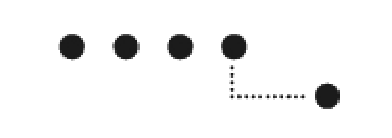
\includegraphics[height=0.875cm,width=3cm]{../../images/logo_BFH.eps}}
\parbox[c]{2.2cm}
{\tiny{\textsf{Berner Fachhochschule \\
Hochschule f�r \\
Technik und Informatik}}}}
\lfoot{}
\cfoot{\textsf{\thepage}}
\rfoot{}
\setlength{\headrulewidth}{0.6pt}
\setlength{\footrulewidth}{0.6pt}
\setlength{\topmargin}{-50pt}
\addtolength{\headheight}{50pt}

\usepackage{colortbl}

\newcommand{\headercol}[2]{\multicolumn{1}{|>{\bfseries\columncolor[gray]{0.82}}p{#1}|}{\textsf{#2}}}
\newcommand{\ace}[0]{\emph{ACE }}



\begin{document}

\setlength{\parindent}{0pt}
\setlength{\parskip}{6pt}

\begin{titlepage}
\thispagestyle{empty}
  
\includegraphics[height=1.5in]{../images/pix.eps}

  \begin{center}

    {\fontsize{40}{45} \textbf{\textsf{ACE}}} \\
    \textsf{a collaborative editor} \\
        
    \vspace{36pt}
        
    {\huge{\textbf{\textsf{}}}} \\

    \vspace{36pt}

	\textsf{Berne University of Applied Sciences} \\
    \textsf{School of Engineering and Information Technology} \\
    
  \end{center}

  \vfill
  
  \begin{tabular}{ll}
   \hline

   \\

   \multicolumn{1}{>{\bfseries}p{1.5in}}{\textsf{Date:}} &
   \multicolumn{1}{>{}p{4.3in}}{\textsf{08.11.2005}}          \\
   
   \\
   
   \multicolumn{1}{>{\bfseries}p{1.5in}}{\textsf{Version:}}     &   
   \multicolumn{1}{>{}p{4.3in}}{\textsf{0.1}}                 \\

   \\
   
   \multicolumn{1}{>{\bfseries}p{1.5in}}{\textsf{Projectteam:}}                 &
   \multicolumn{1}{>{}p{4.3in}}{\textsf{Mark Bigler (biglm2@hta-bi.bfh.ch)}}  \\
   \multicolumn{1}{>{\bfseries}p{1.5in}}{}                                      &
   \multicolumn{1}{>{}p{4.3in}}{\textsf{Simon Raess (rasss@hta-bi.bfh.ch)}}    \\
   \multicolumn{1}{>{\bfseries}p{1.5in}}{}                                      &
   \multicolumn{1}{>{}p{4.3in}}{\textsf{Lukas Zbinden (zbinl@hta-bi.bfh.ch)}} \\   
   
   \\
   
   \multicolumn{1}{>{\bfseries}p{1.5in}}{\textsf{Receivers:}}                       &
   \multicolumn{1}{>{}p{4.3in}}{\textsf{Jean-Paul Dubois (doj@hta-bi.bfh.ch)}}       \\
   \multicolumn{1}{>{\bfseries}p{1.5in}}{}                                          &
   \multicolumn{1}{>{}p{4.3in}}{\textsf{Claude Fuhrer (frc@hta-bi.bfh.ch)}}       \\

   \\
   
   \multicolumn{1}{>{\bfseries}p{1.5in}}{\textsf{Location:}}               &   
   \multicolumn{1}{>{}p{4.3in}}{\textsf{Subversion Repository}} \\

   \\  
   
   \hline
  \end{tabular}

\end{titlepage}


\tableofcontents
\newpage


\section{Introduction}

The \emph{Developers Guide} contains information on how to build the application
from source, how to install, and run the application. Further, information
about the subversion repository is given.

Unless you want to change the source code, we do not recommend to build the
application from source. We provide installers for Windows and a double
clickable application for Mac OS X. These install a completely working
application without the need for all the details that follow.


\section{Setup}
ACE uses Apache Ant (see \href{http://ant.apache.org/}{http://ant.apache.org/})
to build the application. If you have not installed Ant, download and install
it from the above URL. Further, we use a special Ant task to download the
libraries used by ACE. These libraries are not stored inside of the source
repository.

\subsection{Maven 2.0 Ant Tasks}
Maven 2.0 now comes with a set of Ant tasks that can be used to utilise Maven's
artifact handling features from within Ant. This includes most notably the
transitive \emph{Dependency management} handling of Maven 2.0. You can
download these Ant tasks from \\
\href{http://maven.apache.org/download.html}{http://maven.apache.org/download.html}.

\subsubsection{Installation}
To install the Maven Ant tasks you have to do the following:
\begin{itemize}
 \item download the maven-artifact-ant-2.0-dep.jar from the Maven download site
 \item copy the downloaded jar file to the directory \texttt{ANTHOME/lib} where \texttt{ANTHOME} is where Ant is installed
\end{itemize}

\subsubsection{Maven Repositories}
ACE uses two different Maven repository. A Maven repository is a place where
dependencies are installed. The first repository is a custom repository that
stores all dependencies that are not available from the default Maven
repository. The URL of this repository is http://ace.iserver.ch/maven2. The
second repository is the standard Maven repository at the URL
http://repo1.maven.org/maven2/.

\subsubsection{Dependencies}
In the \texttt{build.xml} you find the declaration of the dependencies.

\small{
\begin{verbatim}
<artifact:dependencies pathId="dependency.classpath">
		<dependency groupId="jdom" 
		            artifactId="jdom" 
		            version="1.0"/>
		<dependency groupId="commons-beanutils" 
		            artifactId="commons-beanutils" 
		            version="1.7.0"/>
        ...
</artifact:dependencies>
\end{verbatim}
}

A dependency has a group id, an artifact id, and a version. You have to know
these in order to add dependencies (browse the Maven repositories to find
out the correct values). The dependencies are downloaded to a local repository,
which can be found in the user's home directory in the folder 
\texttt{.m2/repository/}.

The id given to the set of dependencies with the \texttt{pathId} attribute
can be used like any other path in the Ant build file. The Maven Ant tasks
allow to get the correct versions of dependencies without needing to place
them in the source repository.

To find out more about the Maven Ant tasks visit
\href{http://maven.apache.org/ant-tasks.html}{http://maven.apache.org/ant-tasks.html}.

\subsubsection{First Time Build}
When you run the build the first time you will get a couple of messages saying that dependencies are downloaded to the local maven repository. You will get 
some warnings too, because the task first checks the custom
repository of ACE, which does not contain all the dependencies of the project.


\section{Directory Structure}
ACE has the following contents in the top-level directory:

\begin{itemize}
 \item build: the build directory
 \item build.xml: the main build file
 \item dist: distributions
 \item doc: documentation
 \item LICENSE.txt: ACE project license
 \item project.properties: used by Maven
 \item project.xml: Maven project.xml
 \item src: the sources of the project
 \item www: the project website
\end{itemize}

\subsection{Build Products}
The \texttt{build} folder contains the build results of the project:

\begin{itemize}
 \item ant-graph.*: dependency graph of Ant build file
 \item api: javadoc API documentation
 \item build-dependencies.xml: generated build file to copy dependencies
 \item classes: compiled classes from src/java
 \item integration-test: compiled classes from src/integration-test
 \item lib: copied dependency jar files
 \item osx: compiled classes from src/osx as well as built application bundle
 \item resources: copied resources from src/resources
 \item resources-test: copied resources from src/resources-test
 \item stubs: compiled classes from src/stub
 \item test: compiled classes from src/test
 \item testreports: JUnit testreports
\end{itemize}

\subsection{Sources}
The \texttt{src} folder contains the sources of the project.

\begin{itemize}
 \item installer: windows NSIS installer scripts
 \item integration-test: integration tests
 \item java: java sources
 \item osx: OS X customization java code and template for application bundle
 \item resources: runtime resources (images, property files, ...)
 \item resources-test: test resources
 \item stubs: stub classes for testing purpose
 \item test: JUnit tests
 \item test-app: test applications
\end{itemize}

\subsection{Documentation}
The \texttt{doc} folder contains the sources of the project:

\begin{itemize}
 \item developersguide: the \LaTeX{} sources of the developers guide
 \item finalreport: thd \LaTeX{} sources of the final report
 \item images: images for the documentation
 \item latex: \LaTeX{} templates
 \item projectmanual: the \LaTeX{} sources of the project manual
 \item systemrequirements: the \LaTeX{} sources of the system requirements
 \item templates: source code header
 \item usermanual: the \LaTeX{} sources of the user manual
\end{itemize}


\section{Build File}

The Ant build file contains the all the relevant targets.
\begin{figure}[H]
 \centering
 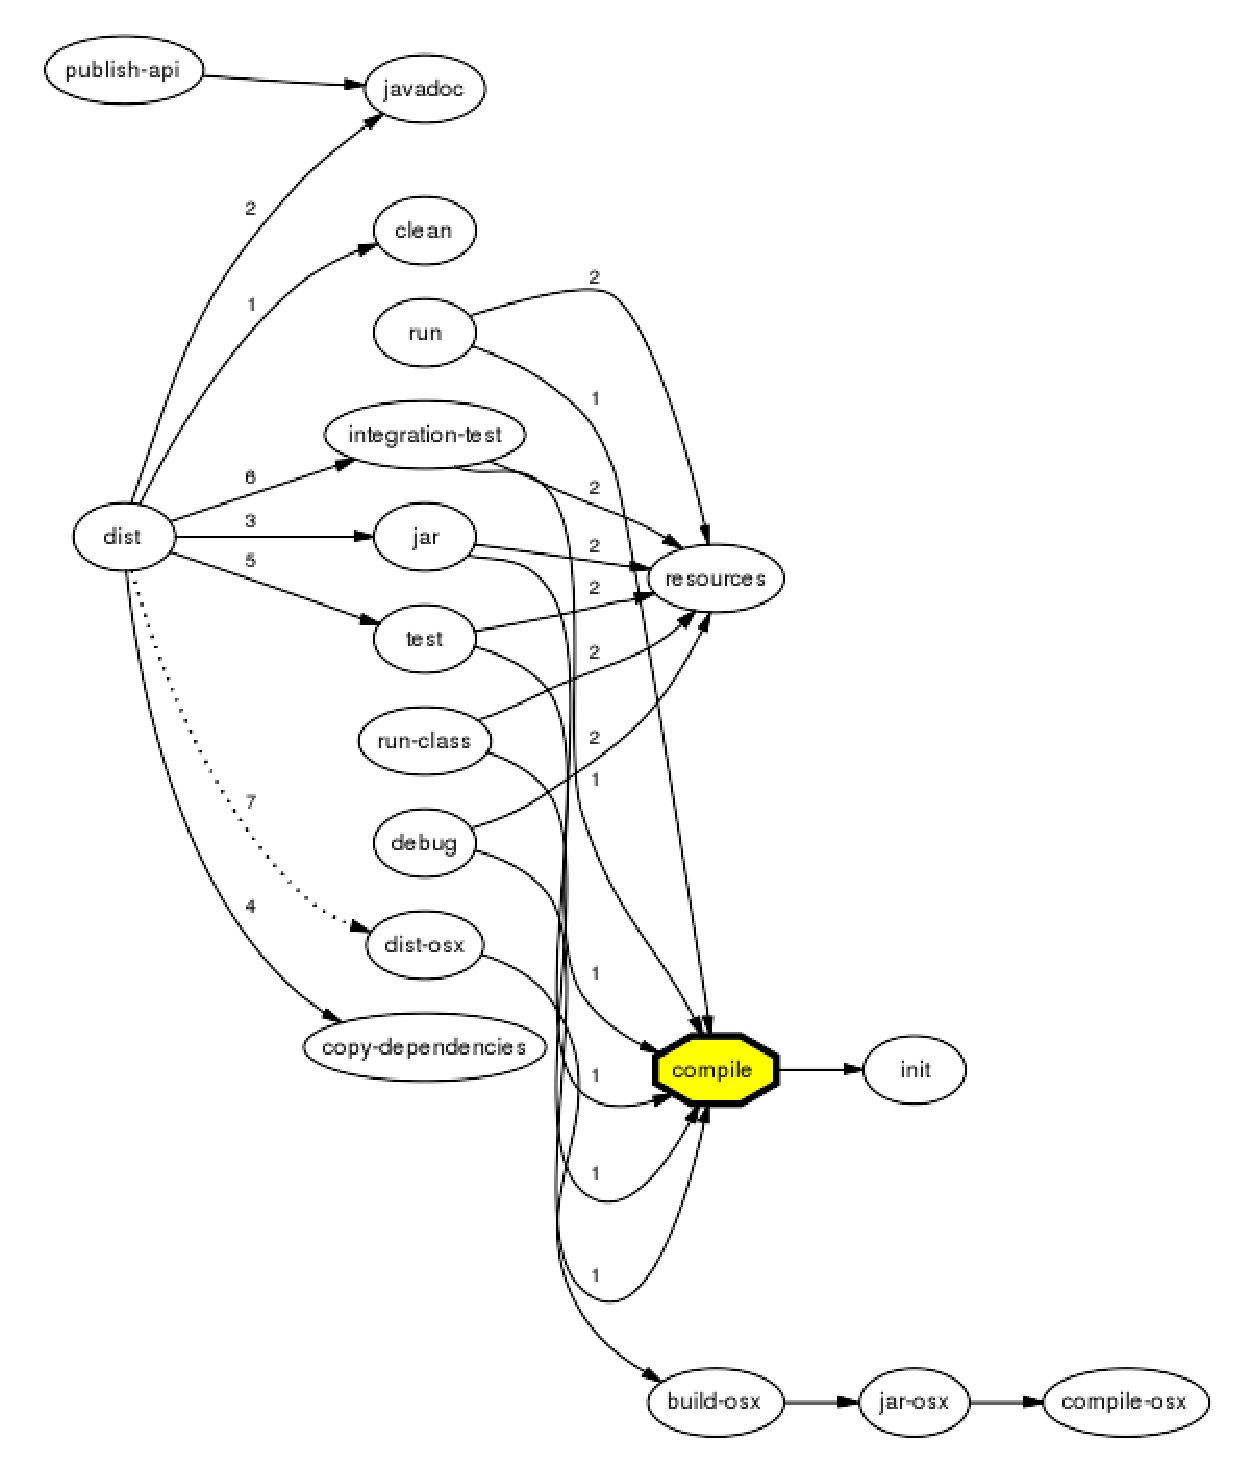
\includegraphics[width=15cm,height=11.6cm]{../images/developersguide/ant-graph.eps}
 \caption{Ant build file dependencies}
\end{figure}

The main targets are:
\begin{itemize}
 \item \texttt{compile}
 \item \texttt{test}
 \item \texttt{integration-test}
 \item \texttt{run}
 \item \texttt{clean}
 \item \texttt{javadoc}
 \item \texttt{dist}
\end{itemize}

\subsection{Compiling the Sources}
To compile the sources you use the Ant target \texttt{compile}. 

\subsection{Running the Tests}
There are two test targets. The first that runs the unit tests is called
\texttt{test}. These tests are run regularly by our continous integration
server. The test sources are found in the directory \texttt{/src/test}. They
must run quickly and deterministically.

The other test target is \texttt{integration-test} which runs integration tests.
Integration tests test large parts of the system and thus run slower than
the pure unit tests.

\subsection{Running the Application}
You can run the application by calling the \texttt{run} task. This starts
the main class of the whole application. If you want to run another class
with the main argument, you can start it with by calling the \texttt{run-class}
task with a system property \texttt{class} set to the correct class name.
You do this from the command line with an additional argument 
\texttt{-Dclass=...}. To debug the application, there is a \texttt{debug}
target that starts the JVM with the correct startup parameters. Connect
your favorite debugger to the JVM. The connection parameters are:
\begin{itemize}
 \item connection type: socket attach
 \item host: localhost
 \item port: 8000
\end{itemize}

\subsection{Cleaning the Build Results}
The \texttt{clean} target can be used to clean the build directory,
forcing a complete rebuild.

\subsection{Javadoc}
The \texttt{javadoc} target creates the Javadoc of the application into the
directory \texttt{/build/api}.

\subsection{Creating a Distribution}
The Ant target \texttt{dist} creates a \texttt{tar.gz} file containing the
sources, the javadoc, and all the necessary jar files into the directory
\texttt{/dist}.


\section{Building the Installers}

The build file has some targets to create OS specific installers. Currently,
there are installers for OS X and Windows.

\subsection{OS X}
The OS X installer is built by the target \texttt{dist-osx}, which is 
called by the standard \texttt{dist} target. The OS X installer can only
be built on OS X for two reasons. First, the targets use a command line
utility only available on OS X and second, the customization Java code
for OS X relies on Apple Java extensions, which are not available on
other systems.

The resulting disk image is placed in the \texttt{dist} folder. The disk
image can be mounted in every version of Mac OS X. The disk image contains
the application bundle.

\subsubsection{Application Bundles}
On Mac OS X, an application is basically a folder containing a specialized
structure, called application bundle. The extension of such an application
bundle is \texttt{.app}. A bundle has the following basic content:

\begin{figure}[H]
 \centering
 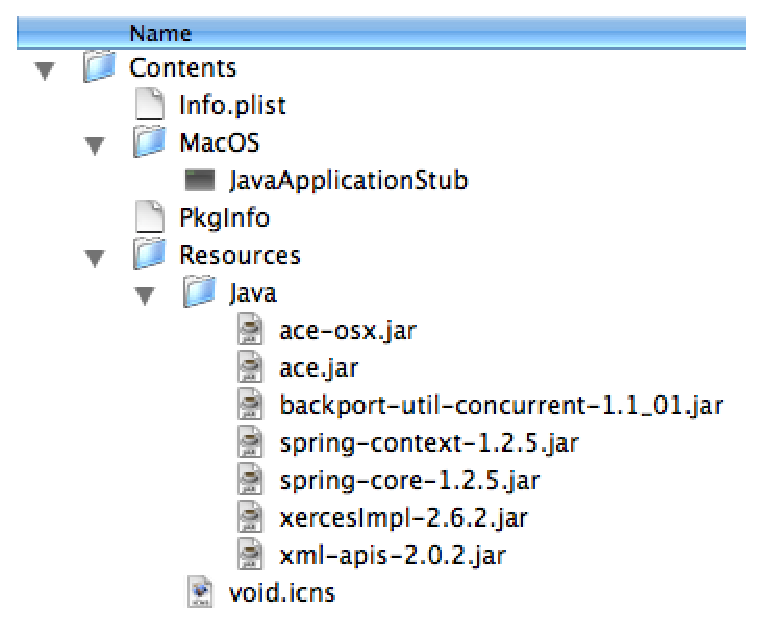
\includegraphics[width=12.3cm,height=10.2cm]{../images/developersguide/app-bundle.eps}
 \caption{application bundle structure}
\end{figure}

The file \texttt{Info.plist} is used by the operating system to determine
things like the executable, the icons for the application, Java version to
use, and the classpath. The \texttt{Resources} folder contains all the
resources needed by the application. In ACE, all the required jar files
are placed inside a subfolder of \texttt{Resources}.

Application bundles can be installed by simply moving the bundle into any
place the user likes. There is no need for an installer. Everything needed
by the application is contained in the bundle. Launching the application
happens by double-clicking the application bundle.

\subsubsection{Ant Targets}
The Ant targets ending with \texttt{osx} are used to build the Mac OS X
application bundle. To do this, a special Ant task is required. The Ant
task is called \texttt{EnhancerTask}. This task determines all the needed
dependency libraries from a fileset. It allows to further exclude some
unwanted dependencies, for instance JUnit libraries by specifying excludes.
This task is needed because we define dependencies as Maven Ant task
dependencies. A dependency can have additional dependencies, which in turn
can have dependencies, and so on. The dependency declaration from 
the Maven Ant task allows to set a fileset attribute, which allows to
get all the needed dependency jar files.

The task must be defined with a \texttt{typedef}:

\small{
\begin{verbatim}
<typedef name="enhance"
         classname="ch.iserver.ace.ant.dependency.EnhancerTask"
         classpathref="enhancer.classpath"/>
\end{verbatim}
}

The enhance task can have two attributes.
\begin{itemize}
 \item source: the source Info.plist file
 \item target: the generated enhanced Info.plist file
\end{itemize}

Further, the enhance task supports nested \texttt{fileset} elements as well
as \texttt{exclude} elements. All the files included by the fileset are
added to the classpath declaration in the \texttt{Info.plist} file, except
for those files that are explicitely excluded by an exclude element.

\small{
\begin{verbatim}
<enhance source="Info.plist" target="Info.plist.enhanced">
  <fileset refid="dependency.fileset"/>
  <exclude name="junit*.jar"/>
</enhance>
\end{verbatim}
}

\end{document}
